\documentclass[xcolor=dvipsnames, 11pt]{beamer}

\usetheme{Warsaw}
\useoutertheme{split}
\setbeamertemplate{headline}{}

\usepackage{ucs}
\usepackage[utf8x]{inputenc}
\usepackage[greek,english]{babel}
\usepackage{hyperref}
\usepackage{tcolorbox}
\usepackage{alphabeta}
\usepackage{amsmath}
\usepackage{amsthm}
\usepackage{caption}
\usepackage{algorithm2e}
\tcbuselibrary{theorems}

\newtcbtheorem{mydefinition}{\el Ορισμός}%
{colback=blue!5,colframe=black!15!black,fonttitle=\bfseries}{th}

\newtcbtheorem{mytheorem}{\el Θεώρημα}%
{colback=blue!5,colframe=black!15!black,fonttitle=\bfseries}{th}

\newtcbtheorem[number within=section]{mylemma}{Λήμμα}%
{colback=blue!5,colframe=black!15!black,fonttitle=\bfseries}{th}

\newcommand{\en}{\selectlanguage{english}}
\newcommand{\el}{\selectlanguage{greek}}
\newcommand{\R}{\mathbb{R}}

\setbeamertemplate{itemize items}[ball]
\setbeamertemplate{itemize subitem}[ball]

\begin{document}

\title{Travelling Salesman Problem}
\subtitle{TSP}

\author[\el Σιώρος Βασίλειος, Ανδρινοπούλου Χριστίνα]{\el Σιώρος Βασίλειος \and \el Ανδρινοπούλου Χριστίνα}
\date{\el Απρίλιος, 2020}

\frame{\titlepage}

\begin{frame}
	\frametitle{\el Δομή Παρουσίασης}
	\footnotesize
	\tableofcontents
\end{frame}

\section{Εισαγωγή}
\begin{frame}
	\frametitle{\el Εισαγωγή}
	\footnotesize
	\tableofcontents[currentsection]
\end{frame}

\subsection{Ορισμός}
\begin{frame}
	\frametitle{\el Ορισμός}
	\begin{itemize}
		\item \el Κλασσικό πρόβλημα της θεωρητικής επιστήμης των  υπολογιστών. 
		\item \el Ο πωλητής οφείλει να επισκευτεί \en n \el το πλήθος πόλεις για να πουλήσει το εμπόρευμά του.  
		\item \el Ο πωλητής πρέπει να επισκεφτεί την κάθε πόλη ακριβώς μία φορά ακολουθώντας το συντομότερο δρομολόγιο και να επιστρέψει στην πόλη εκκίνισης.
	\end{itemize}
	\begin{figure}
		
\includegraphics[scale=0.3]{images/tsp.png}
		\caption{\en Travelling Salesman Problem - TSP. Πηγή: \en \url{https://www.localsolver.com/docs/last/exampletour/tsp.html}}
	\end{figure}
\end{frame}

\subsection{Εφαρμογές}
\begin{frame}
	\frametitle{\el Εφαρμογές}
	\begin{itemize}
		\item \el Μεταφορές και \en Logistics:
		\begin{itemize}
			\item \el Καθορισμός δρομολογίων σχολικών λεωφορείων
			\item \el Παράδοση τροφίμων σε άτομα που δεν μπορούν να μετακινηθούν από το σπίτι
			\item \el Δρομολόγηση φορτηγών για παραλαβή δεμάτων
			\item \el Εφοδιασμός σε ορόφους καταστημάτων ή σε αποθήκες
		\end{itemize}
		\item \el Βιολογία:
		\begin{itemize}
			\item \en DNA sequencing: οι "πόλεις" είναι DNA strings και η απόσταση είναι τα αποτελέσματα μέτρων σημασιολογικής ομοιότητας
		\end{itemize}
		\item \el Διάστημα:
		\begin{itemize}
			\item \el Ελαχιστοποίηση των καυσίμων που απαιτούνται για την παρατήρηση ουράνιων αντικειμένων
		\end{itemize}	
	\end{itemize}
\end{frame}

\section{Θεωρητική Προσέγγιση}
\subsection{Πολυπλοκότητα}
\begin{frame}
	\frametitle{\el Θεωρητική Προσέγγιση}
	\footnotesize
	\tableofcontents[currentsubsection]
\end{frame}

\begin{frame}
	\frametitle{\el Πολυπλοκότητα}
	\begin{figure}
		
\includegraphics[scale=0.3]{images/complexity_classes.png}
		\caption{\en P \el κλάση και \en NP \el κλάση \\ πηγή: \en \url{https://jcaip.github.io/Reduction-and-Intractibility/}}
	\end{figure}
\end{frame}

\begin{frame}
	\frametitle{\el Πολυπλοκότητα}
	\begin{mylemma}{TSP}{}
		Tο πρόβλημα του περιοδεύοντος πωλητή ανήκει στην κλάση NP.	
	\end{mylemma}
	\begin{mylemma}{TSP}{}
		Tο πρόβλημα του περιοδεύοντος πωλητή είναι NP-complete.	
	\end{mylemma}
	\begin{itemize}
		\item \el Δεν περιμένουμε αλγόριθμο που να επιλύει το πρόβλημα σε πολυωνυμικό χρόνο , αλλά κάποιον προσεγγιστικό αλγόριθμο.
	\end{itemize}
\end{frame}

\subsection{Γραφοθεωρητική Προσέγγιση}
\begin{frame}
	\frametitle{\el Θεωρητική Προσέγγιση}
	\footnotesize
	\tableofcontents[currentsubsection]
\end{frame}

\begin{frame}
	\frametitle{\el Γραφοθεωρητική Προσέγγιση}
	\begin{itemize}
		\item \el Το \en TSP \el είναι μία επέκταση του προβλήματος εύρεσης κυκλώματος \en Hamilton.
		\item \el Το \en TSP \el αναζητά ένα κύκλωμα \en Hamilton \el με ελάχιστο μήκος.
		\item \el Θεωρούμε το γράφημα του χαρτη των πόλεων και των αντίστοιχων διαδρομών να είναι το \(G = (V,E,w(i,j))\)
		\item \el \(V\): πόλεις (κορυφές)
		\item \el \(E\) : διαδρομές μεταξύ δύο πόλεων (ακμές) 
		\item \el \(w\): μήκος διαδρομής από την πόλη \(i\) στην πόλη \(j\) (το βάρος της ακμής \((i,j)\))
		
		\begin{align}
		w:E \rightarrow \R^{+}
		\end{align} 	
		τέτοια ώστε να ισχύει 
		\begin{align}
		w(i,k) \leq w(i,j) + w(j,k)
		\end{align} 
	\end{itemize}
\end{frame}

\subsection{Γεωμετρική Προσέγγιση}
\subsubsection{Αλγόριθμος Σύγκρισης Γωνιών}
\begin{frame}
	\frametitle{\el Θεωρητική Προσέγγιση}
	\footnotesize
	\tableofcontents[currentsubsection]
\end{frame}

\begin{frame}
	\frametitle{\el Γεωμετρική Προσέγγιση - Αλγόριθμος Σύγκρισης Γωνιών}
	\begin{itemize}		
		\item \el  Πρώτο βήμα: εύρεση του κυρτού περιβλήματος των σημείων 
		\item \el Το κυρτό περίβλημα είναι μία πρώτη μορφή του τελικού μονοπατιού \en ("partial μονοπάτι").
	\end{itemize}
	\begin{figure}
		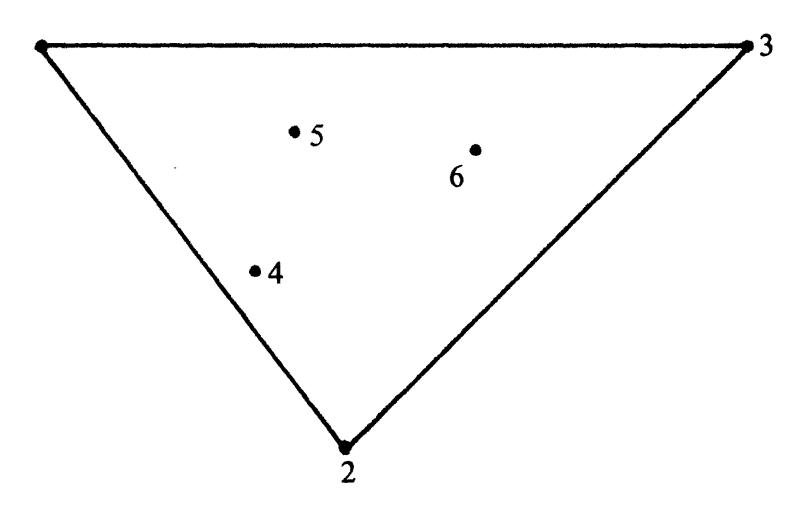
\includegraphics[scale=0.2]{images/geometric_approach_angle1.png}
		\caption{Οι "εσωτερικές" πόλεις είναι τα σημεία με label 4,5 και 6. Οι "εξωτερικές" πόλεις βρίσκονται στο convex hull (partial μονοπάτι)\\ πηγή: \cite{16}}
	\end{figure} 
\end{frame}

\begin{frame}
	\frametitle{\el Γεωμετρική Προσέγγιση - Αλγόριθμος Σύγκρισης Γωνιών}
	\begin{itemize}		
		\item \el Δεύτερο βήμα: ενσωμάτωση των εσωτερικών πόλεων στο μονοπάτι.
		\begin{itemize}		
			\item \el Σχηματίζουμε όλες τις γωνίες των οποίων η κορυφή είναι ένα από τα εσωτερικά σημεία και οι δύο αντίστοιχες πλευρές βαίνουν από δύο διαδοχικά σημεία του \en convex hull.
			\item \el Επιλέγεται η γωνία που έχει το μεγαλύτερο μέτρο.
			\item \el Η αντίστοιχη κορυφή - πόλη ενσωματώνεται στο μονοπάτι μαζί με τις δύο πλευρές της γωνίας
		\end{itemize}
		\item \el Διαδοχικές επαναλήψεις μέχρι να έχουν ενσωματωθεί στο μονοπάτι όλες οι εσωτερικές πόλεις.
	\end{itemize}
	\begin{columns}
		\begin{column}{0.3\textwidth}
			\begin{figure}
				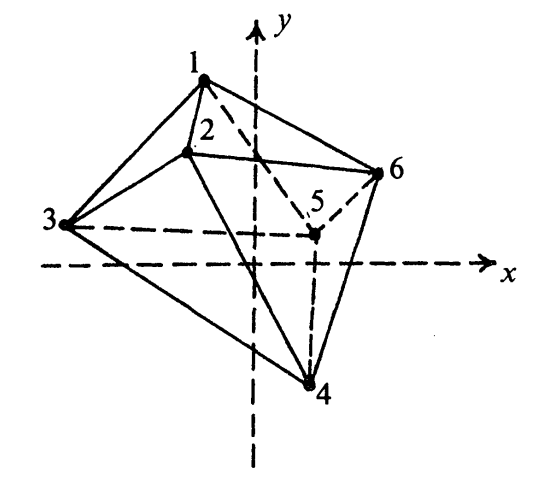
\includegraphics[scale=0.12]{images/geometric_approach_angle2.png}
				\caption{Γωνίες των εσωτερικών πόλεων. Πηγή: \cite{16}}
			\end{figure} 
		\end{column}
		\begin{column}{0.3\textwidth}
			\begin{figure}
				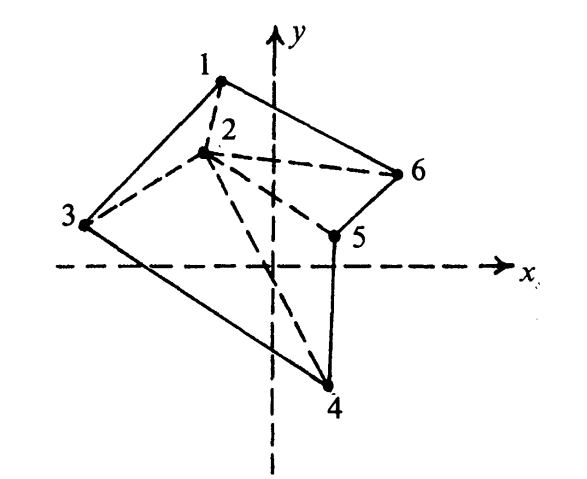
\includegraphics[scale=0.12]{images/geometric_approach_angle3.png}
				\caption{Μεγαλύτερη γωνία: σημείο 5. Πηγή: \cite{16}}
			\end{figure} 
		\end{column}
		\begin{column}{0.3\textwidth}
			\begin{figure}
				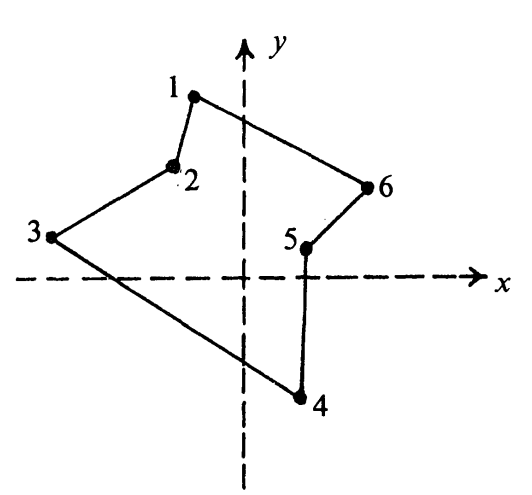
\includegraphics[scale=0.12]{images/geometric_approach_angle4.png}
				\caption{Τελικό μονοπάτι. Πηγή: 	\cite{16}}
			\end{figure} 
		\end{column}	
	\end{columns}
\end{frame}

\begin{frame}
	\frametitle{\el Γεωμετρική Προσέγγιση - Αλγόριθμος Σύγκρισης Γωνιών}
	\begin{figure}
		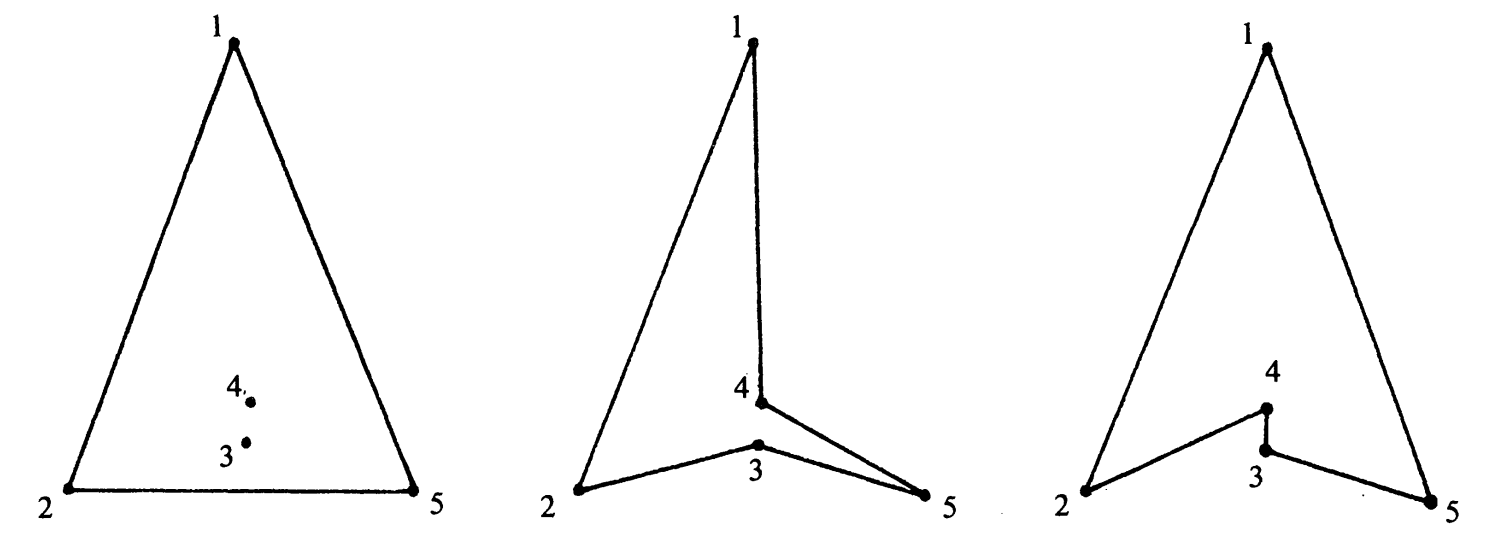
\includegraphics[scale=0.2]{images/geometric_approach_angle5.png}
		\caption{Παράδειγμα παραγωγής μη βέλτιστου μονοπατιού. Ο αλγόριθμος δίνει το αποτέλεσμα που φαίνεται στη μέση, ενώ το βέλτιστο αποτέλεσμα φαίνεται στα δεξία.\\ πηγή: \cite{16}}
	\end{figure}
\end{frame}

\subsubsection{Αλγόριθμος Σύγκρισης Ελλείψεων}
\begin{frame}
	\frametitle{\el Θεωρητική Προσέγγιση}
	\footnotesize
	\tableofcontents[currentsubsection]
\end{frame}
\begin{frame}
	\frametitle{\el Γεωμετρική Προσέγγιση - Αλγόριθμος Σύγκρισης Ελλείψεων}
	\begin{itemize}
		\item \el Εύρεση του \en convex hull (partial μονοπάτι).
		\item \el  Σε κάθε επανάληψη ενσωματώνεται μόνο μία καινούρια εσωτερική πόλη στο μονοπάτι
		\item \el Ο αλγόριθμος τερματίζει όταν όλες οι εσωτερικές πόλεις περιέχονται στο μονοπάτι του πλανόδιου πωλητή. \\
		\item \el Η επιλογή της πόλης που θα ενσωματωθεί στο \en partial \el μονοπάτι γίνεται με τη βοήθεια ελλείψεων.
	\end{itemize}
\end{frame}

\begin{frame}
	\frametitle{\el Γεωμετρική Προσέγγιση - Αλγόριθμος Σύγκρισης Ελλείψεων}
	\begin{itemize}
		\item \el Σε κάθε επανάληψη δημιουργούνται όλες οι ελλείψεις που έχουν εστίες δύο διαδοχικά σημεία του \en convex hull \el και βαίνουν από ένα εσωτερικό σημείο.
		\item \el Για κάθε μία από τις ελλείψεις υπολογίζεται η εκκεντρότητά της.
		\item \el  Επιλέγεται το σημείο που ανήκει στην έλλειψη με τη μεγαλύτερη εκκεντρότητα (λιγότερο κυκλική μορφή).
	\end{itemize}
	\begin{figure}
		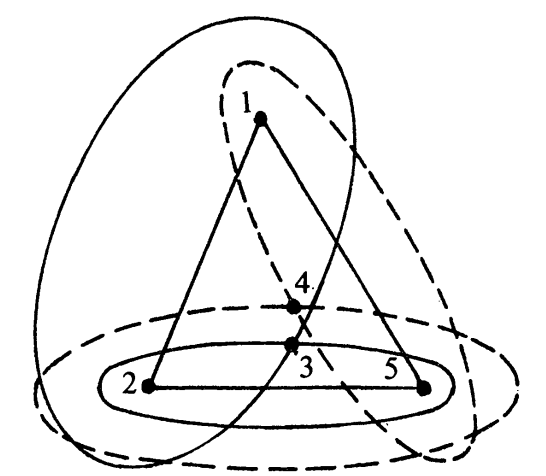
\includegraphics[scale=0.15]{images/geometric_approach_ellipse2.png}
		\caption{Στη φάση αυτή επιλέγεται το εσωτερικό σημείο με label 3, διότι ανήκει στην έλλειψη με τη μεγαλύτερη εκκεντρότητα.\\ πηγή: \cite{16}}
	\end{figure}  
\end{frame}

\begin{frame}
	\frametitle{\el Γεωμετρική Προσέγγιση - Αλγόριθμος Σύγκρισης Ελλείψεων}
	\begin{itemize}
		\item \el Εκκεντρότητα:
		\begin{align*}
		e = \frac{d_3}{d_1 + d_2}
		\end{align*}
		όπου \(d_3\) είναι η απόσταση μεταξύ των δύο εστιών και \(d_1, d_2\) είναι η απόσταση μεταξύ ενός σημείου της έλλειψης και των δύο εστιών αντίστοιχα.
	\end{itemize}
	\begin{figure}
		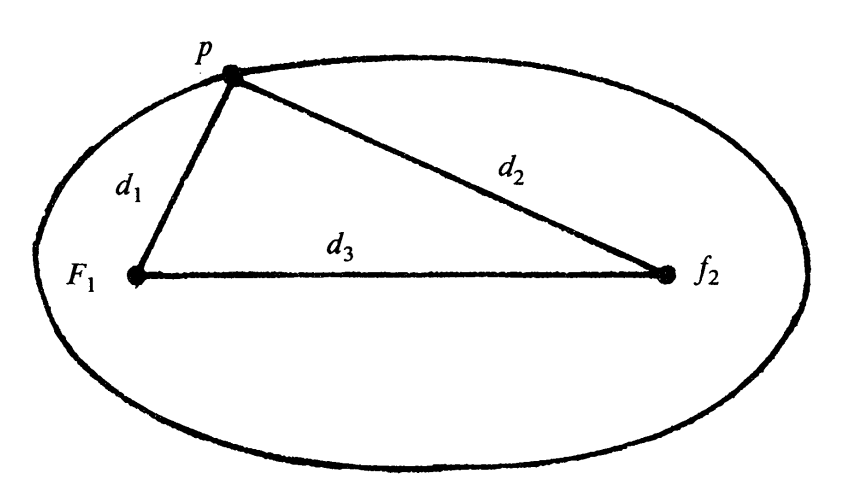
\includegraphics[scale=0.2]{images/geometric_approach_ellipse1.png}
		\caption{Η εκκεντρότητα δίνεται από τον τύπο \(e = \frac{d_3}{d_1 + d_2}\)\\ πηγή: \cite{16}}
	\end{figure}
\end{frame}

\subsubsection{Αλγόριθμος με τριγωνοποίηση Delaunay}
\begin{frame}
	\frametitle{\el Θεωρητική Προσέγγιση}
	\footnotesize
	\tableofcontents[currentsubsection]
\end{frame}

\begin{frame}
	\frametitle{\el Γεωμετρική Προσέγγιση - Αλγόριθμος με τριγωνοποίηση \en Delaunay}
	\begin{itemize}
		\item \el Οι πόλεις παιρνούν από τη διαδικασία της τριγωνοποίησης \en Delaunay.
		\item \el Κατασκευάζεται ένα αρχικό μονοπάτι που περιέχει το \en convex hull.
		\item \el Σε κάθε επανάληψη:
		\begin{itemize}
			\item \el Διαγράφεται κάποια ακμή \(E_{mn}\) του αρχικού μονοπατιού και στη θέση της εισάγονται δύο νέες.
			\item \el Οι δύο νέες ακμές συνδέουν συνδέουν τις πόλεις \(C_m\) και \(C_n\) με την πόλη που βρίσκεται στα αριστερά τους (αν δεν περιέχεται ήδη στο μονοπάτι).
		\end{itemize}
		\item \el Αφού, ο αλγόριθμος επεκτείνεται προς τις πόλεις που βρίσκονται στα αριστερά, μία εύλογη επιλογή για αρχική διαδρομή θα ήταν το \en convex hull \el των σημείων με \en CCW \el σειρά.
		\item \el Ο αλγόριθμος μπορεί να λειτουργήσει και με φορά προς τα δεξιά με αντίστοιχο τρόπο.
	\end{itemize}
\end{frame}

\begin{frame}
	\frametitle{\el Γεωμετρική Προσέγγιση - Αλγόριθμος με τριγωνοποίηση \en Delaunay}
	\begin{itemize}
		\item \el Πώς επιλέγεται ποια ακμή θα διαγραφεί\en ;
		\begin{itemize}
			\item \el  Μία ακμή επιλέγεται να διαγραφεί, έναντι των άλλων, σύμφωνα με την ποιότητά της \(Q_{mn}\).
			\item \el Το \(Q_{mn}\) υπολογίζεται με βάση το μήκος της ακμής και το μήκος των νεοεισαχθέντων ακμών.
		\end{itemize}
	\end{itemize}
\end{frame}

\begin{frame}
	\frametitle{\el Γεωμετρική Προσέγγιση - Αλγόριθμος με τριγωνοποίηση \en Delaunay}
	\begin{itemize}
		\item \el Οι αλγόριθμοι επίλυσης του \en TSP \el με τη βοήθεια της \en Delaunay \el τριγωνοποίησης δεν παράγουν το βέλτιστο μονοπάτι.
		\item \el  Tο βέλτιστο μονοπάτι δεν είναι πάντοτε ένα υποσύνολο του \en Delaunay \el γράφου.
	\end{itemize}
	\begin{figure}
		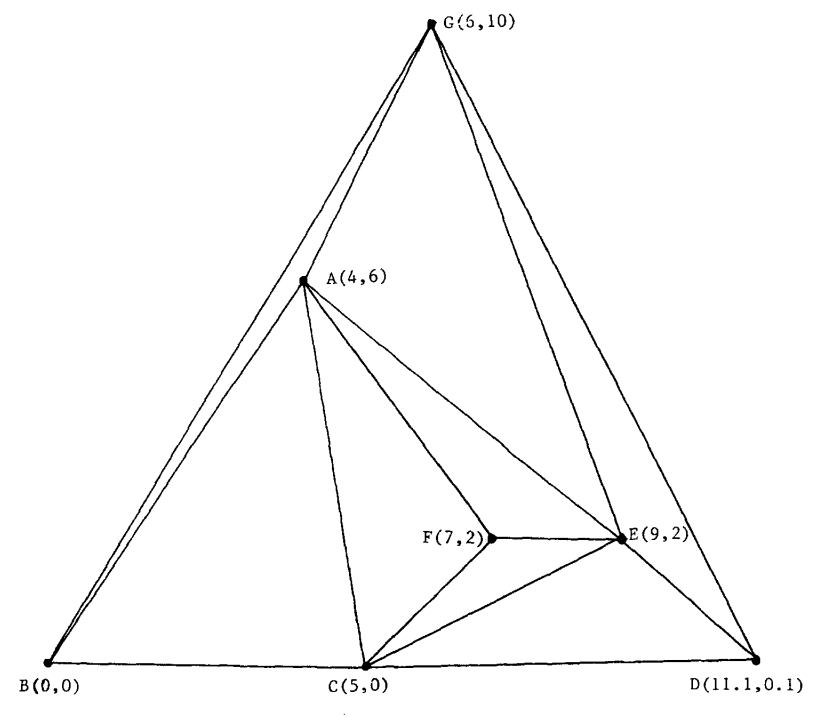
\includegraphics[scale=0.14]{images/delaunay.png}
		\caption{Οπτικό παράδειγμα \en TSP \el σε τριγωνοποιημένο γράφο \\ πηγή: \cite{18}}
	\end{figure} 
\end{frame}

\subsection{Ειδικές Περιπτώσεις \en TSP}
\subsubsection{Convex Hull and Line TSP}
\begin{frame}
	\frametitle{\el Θεωρητική Προσέγγιση}
	\footnotesize
	\tableofcontents[currentsubsection]
\end{frame}

\begin{frame}
	\frametitle{Convex Hull and Line TSP}
	\begin{itemize}
		\item \el Ειδική περίπτωση του Ευκλείδιου \en TSP
		\item \el Οι πόλεις χωρίζονται σε δύο κατηγορίες:
		\begin{itemize}
			\item \el Πρώτη κατηγορία: \(m\) το πλήθος πόλεις - σημεία τα οποία δημιουργούν ένα ευθύγραμμο τμήμα.
			\begin{itemize}
				\item \el Συμβολίζονται με \(g_i\).
			\end{itemize}
			\item \el Δεύτερη κατηγορία: \(n\) το πλήθος πόλεις - σημεία τα οποία δημιουργούν ένα κυρτό περίβλημα, που περιβάλλει τα \(m\) σημεία - πόλεις της πρώτης κατηγορίας.
			\item \el Διακρίνονται σε δύο κατηγορίες:
			\begin{itemize}
				\item \el Τα σημεία που βρίσκονται πάνω από την ευθεία \(G\) και συμβολίζονται με \(u_i\).
				\item \el Τα σημεία που βρίσκονται κάτω από την ευθεία \(G\) και συμβολίζονται με \(l_i\).
			\end{itemize}
		\end{itemize}
	\end{itemize}
\end{frame}

\begin{frame}
	\frametitle{Convex Hull and Line TSP}
	\begin{figure}
		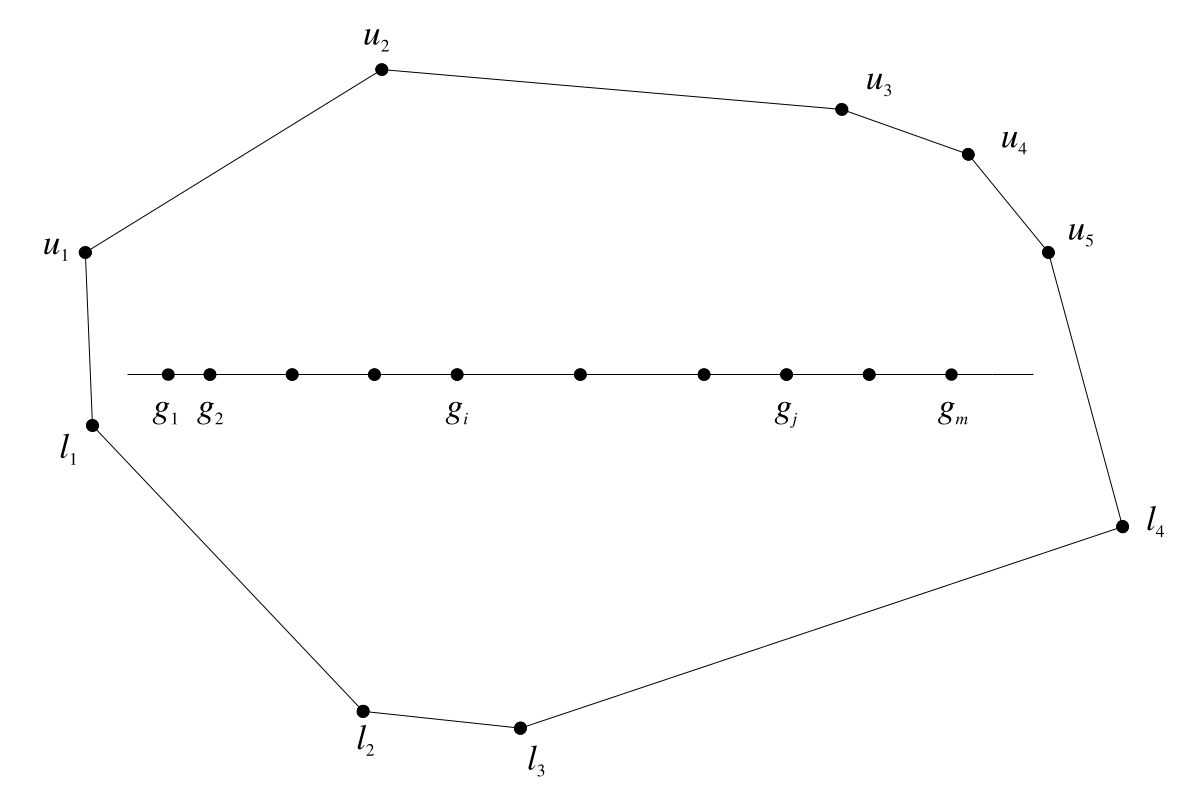
\includegraphics[scale=0.2]{images/ConvexHullLineTSP1.png}
		\caption{Οπτικό παράδειγμα ενός στιγμιοτύπου Convex Hull and Line TSP \\ πηγή: \cite{17}}
	\end{figure}   
\end{frame}

\begin{frame}
	\frametitle{Convex Hull and Line TSP}
	\begin{itemize}
		\item \el Θεμελιώδεις παραδοχές:
		\begin{itemize}
			\item \el Το βέλτιστο μονοπάτι δεν διασταυρώνεται με τον εαυτό του.
			\item \el Το μονοπάτι ακολουθεί μία κυκλική διαδρομή μίας κατεύθυνσης, ώστε να μην υπάρξουν πιθανές διασταυρώσεις.
			\item \el Σε κατάλληλο σημείο, δηλαδή ανάμεσα σε δύο γειτονικές πόλεις του \en convex hull \el ενσωματώνονται οι πόλεις που ανήκουν στο σύνολο \(G\).
		\end{itemize}
	\end{itemize} 
\end{frame}

\begin{frame}
	\frametitle{Convex Hull and Line TSP}
	\begin{itemize}
		\item \el Ποιοι γείτονες είναι κατάλληλοι για την εισαγωγή των εσωτερικών πόλεων \en ;
	\end{itemize} 
	\begin{mydefinition}{Αποδεκτοί γείτονες}{}
		Δύο σημεία \(v,w \in B\) καλούνται αποδεκτοί γείτονες και μεταξύ τους μπορεί να παρεμβληθεί παράκαμψη μονοπατιού που πειέχει το σύνολο των πόλεων \(\left\{g_i,...,g_j\right\}\), όπου \(1 \leq i < j \leq m\) αρκεί να ισχύει μία από τις παρακάτω συνθήκες: \\
		1. Τα σημεία \(v,w\) βρίσκονται (και τα δύο) είτε πάνω από την ευθεία G, είτε κάτω από αυτήν ή \\
		2. \(\left\{v,w\right\} = \left\{u_p, l_p\right\}\) και \(j = m\) ή \\
		3. \(\left\{v,w\right\} = \left\{u_1, l_1\right\}\) και \(i = 1\) 
	\end{mydefinition} 
\end{frame}

\subsubsection{Time Window TSP}
\begin{frame}
	\frametitle{\el Θεωρητική Προσέγγιση}
	\footnotesize
	\tableofcontents[currentsubsection]
\end{frame}

\begin{frame}
	\frametitle{Time Window TSP}
	\begin{itemize}
		\item \el Κλασσικό \en TSP \el με επιπλέον περιορισμούς:
		\begin{itemize}
			\item \el Κάθε σημείο επίσκεψης \(v\) \el έχει ένα χρονικό \en deadline \(D(v)\).
			\item \el Κάθε σημείο επίσκεψης \(v\) χαρακτηρίζεται από έναν χρόνο ελευθέρωσης \en (release time) \(R(v)\).
			\item \el Ο πωλητής μπορεί να επισκεφτεί ένα σήμειο μόνο εντός του χρονικού πλαισίου \([R(v), D(v)]\). 
		\end{itemize}
		\item \el Στόχος: ελαχιστοποιήση της απόστασης που διανύεται από τον πωλητή
		\item \el Ο πωλητής είναι υποχεωμένος να επισκεφτεί όλες τις πόλεις, την κάθε μία εντός του επιτρεπτού χρονικού πλαισίου.
	\end{itemize}
\end{frame}

\begin{frame}
	\frametitle{Time Window Prize Collecting}
	\begin{itemize}
		\item \el Κάθε πόλη χαρακτηρίζεται από ενα \en release time \el και ένα \en deadline.
		\item \el Ο πλανόδιος πωλητής δεν είναι υποχρεωμένος να επισκεφτεί όλες τις πόλεις.
		\item \el Κάθε φορά που επισκέπτεται μία πόλη εντός του επιτρεπτού χρονικού διαστήματος, τότε λαμβάνει μία επιβράβευση.
		\item \el Στόχος: μεγιστοποίηση της επιβράβευση.
	\end{itemize}
\end{frame}

\begin{frame}
	\frametitle{Time Window TSP - \en 1D}
	\begin{itemize}
		\item \el Οργανώνουμε τα δεδομένα χώρου (σημεία - πόλεις) και χρόνου \en (time windows) \el σε ένα σύστημα συντεταγμένων \(tx\).
		\item Οριζόντιος άξονας: χρόνος
		\item \el Κατακόρυφος άξονας: θέσεις των σημείων προς επίσκεψη
		\item \el Τα \en time windows \el έχουν τη μορφή οριζόντιων ευθύγραμμων τμημάτων και συμβολίζονται με \(σ_i\) για την πόλη \(v_i\).
	\end{itemize}
	\begin{figure}
		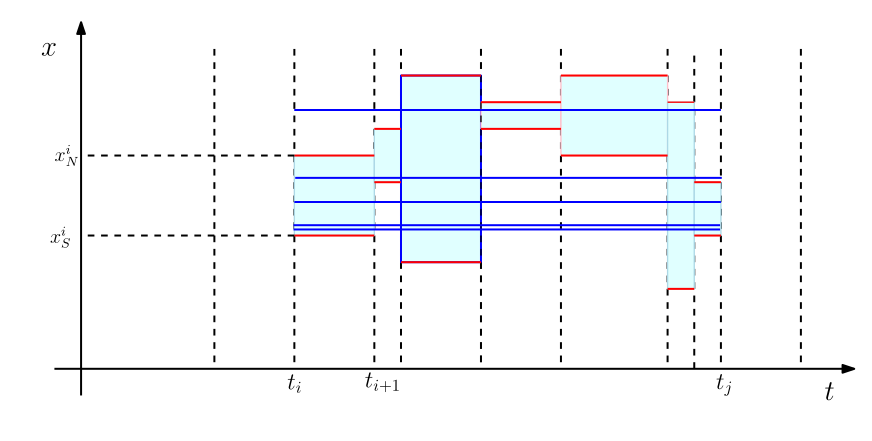
\includegraphics[scale=0.18]{images/presetationimage.png}
		\caption{Καταγραφή χωρικής και χρονική πληροφορίας στην περίπτωση 1D TWTSP \\ πηγή: \cite{1}}
	\end{figure}
\end{frame}

\begin{frame}
	\frametitle{Time Window TSP - \en 1D - \el 'Απειρη Ταχύτητα}
	\begin{mytheorem}{TWTSP - 1D}{}
		Για ένα TWTSP σε μία διάσταση με όριο ταχύτητας \(s = \infty\) και \(L_{max}\) να είναι το μέγιστο μήκος ευθύγραμμου τμήματος \(σ\), για οποιοδήποτε \(ε > 0\) μπορούμε να βρούμε μονοπάτι \(P\) σε χρόνο \(Ο(n^{O(\frac{\log L_{max}}{\log 1 + ε})} \log L_{max})\) τέτοιο ώστε: \\
		1. Το μήκος του \(P\) να είναι το πολύ όσο το μήκος του βέλτιστου μονοπατιού και \\
		2. Ο πωλητής επισκέπτεται κάθε \(σ_i\) σε χρόνο \([r_i - εL_i, d_i + εL_i]\). 
	\end{mytheorem}
\end{frame}

\begin{frame}
	\frametitle{Time Window TSP - \en 1D - \el Πεπερασμένη Ταχύτητα}
	\begin{mytheorem}{TWPC - 1D}{}
		Για ένα TWPC σε μία διάσταση με περιορισμένο όριο ταχύτητας \(s\) και \(L_{max}\) να είναι το μέγιστο μήκος ευθύγραμμου τμήματος \(σ\), υποθέτοντας ότι το μικρότερο time window έχει μήκος μεγαλύτερο ή ίσο με 1, τότε για οποιοδήποτε \(ε > 0\) μπορούμε να βρούμε μονοπάτι \(P\) σε χρόνο \(Ο((nL_{max})^{O(\frac{\log L_{max}}{\log 1 + ε})})\) τέτοιο ώστε: \\
		1. Το πλήθος των ευθυγράμμων τμημάτων που περιέχονται στο \(P\) να είναι τουλάχιστον όσα και στο βέλτιστο μονοπάτι και \\
		2. Ο πωλητής επισκέπτεται κάθε \(σ_i\) σε χρόνο \([r_i - εL_i, d_i + εL_i]\). 
	\end{mytheorem}
	\begin{itemize}
		\item \el Παρόμοια αποτελέσματα ισχύουν και για το \en TWTSP.
	\end{itemize}
\end{frame}

\begin{frame}
	\frametitle{Time Window TSP στο χώρο}
	\begin{itemize}
		\item \el Γενική περίπτωση: οι πόλεις προς επίσκεψη βρίσκονται σε κάποιον χώρο, όπου ισχύει μία μετρική δ.
		\item \el Υποθέτουμε ότι ο πωλητής μας μπορεί να κινείται με μία ταχύτητα \(s\) που ξεπερνά κάποιο \en threshold \el ταχύτητας \(s_{min}\).
		\item \el Αν η ταχύτητά του είναι μικρότερη από αυτήν, τότε θεωρούμε ότι το πρόβλημα δεν έχει εφικτή λύση.
		\item \el Παρουσιάζεται ένας (α,β)-προσεγγιστικός αλγόριθμος.
		\item \el Τα α και β αναφέρονται στην ταχύτητα και το μήκος του μονοπατιού αντίστοιχα.
		\item \el Ο αλγόριθμος ικανοποιεί τις παρακάτω σχέσεις:
		\begin{align*}
		\text{ ταχύτητα} \leq αs \\
		\text{ μήκος μονοπατιού} \leq βλ^{*}(s)
		\end{align*}
	\end{itemize}
\end{frame}

\begin{frame}
	\frametitle{Time Window TSP στο χώρο}
	\begin{itemize}
		\item \el Τα \en release times \el είναι ακέραιοι αριθμοί
		\item \el Κάθε \en time window \el έχει μέγεθος είτε μονάδα, είτε \([0,L]\), όπου \(L\) κάποιος ακέραιος αριθμός.
		\item \el Οι πόλεις που έχουν \en time window \el μεγέθους 1 χρωματίζονται με κόκκινο χρώμα.
		\item \el Οι πόλεις που έχουν \en time window \el \([0,L]\) χρωματίζονται με μαύρο χρώμα. 
		\item \el Για κάθε \(i \leq L\) υπάρχει τουλάχιστον μία κόκκινη πόλη τέτοια ώστε να έχει \en time window \([i-1,i]\).
	\end{itemize}
\end{frame}

\begin{frame}
	\frametitle{Time Window TSP στο χώρο}
	\begin{itemize}
		\item \el Ο πωλητής ξεκινάει από μία κόκκινη πόλη με \en time window \([0,1]\)
		\item \el Επισκέπτεται τις γειτονικές μαύρες πόλεις, κάνοντας ένα <<μαύρο κύκλο>>, και επιστρέφει στην πρώτη κόκκινη πόλη που επισκέφτηκε.
		\item \el Συνεχίζει με τις υπόλοιπες κόκκινες πόλεις με \en time window \([0,1]\).
		\item \el Πηγαίνει σε μία κόκκινη πόλη που έχει \en time window \([1,2]\) \el κ.ο.κ. μέχρι να επισκεφτεί κάθε πόλη. 
	\end{itemize}
	\begin{figure}
		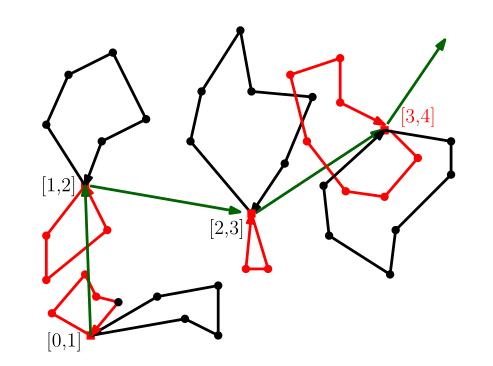
\includegraphics[scale=0.2]{images/twtspd.png}
		\caption{TWTSP - Μαύρος και κόκκινος χρωματισμός πόλεων. Πηγή: \cite{12}}
	\end{figure}
\end{frame}

\section{Υλοποίηση}
\begin{frame}
	\frametitle{\el Υλοποίηση}
	\footnotesize
	\tableofcontents[currentsubsection]
\end{frame}

\begin{frame}
	\frametitle{\el Υλοποίηση \en - TSP}
	\begin{columns}[t]
		\column{.4\textwidth}
		\includegraphics[width=\columnwidth,height=2.8cm]{images/img/separate/tsp/convex_hull_040_1927_068.png}
		\captionof{figure}{Convex Hull}
		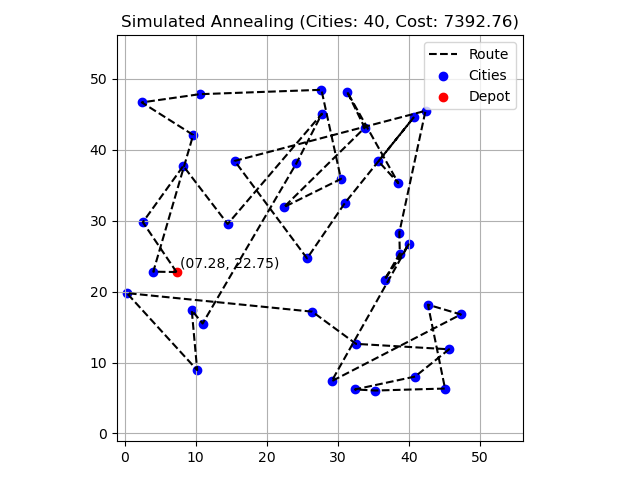
\includegraphics[width=\columnwidth,height=2.8cm]{images/img/separate/tsp/simulated_annealing_040_7392_075.png}
		\captionof{figure}{Simulated Annealing}
		\column{.4\textwidth}
		\includegraphics[width=\columnwidth,height=2.8cm]{images/img/separate/tsp/nearest_neighbor_040_4484_021.png}
		\captionof{figure}{Nearest Neighbor}
		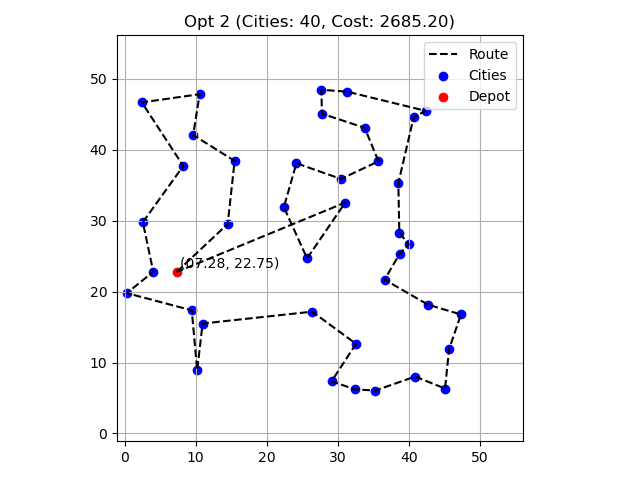
\includegraphics[width=\columnwidth,height=2.8cm]{images/img/separate/tsp/opt_2_040_2685_019.png}
		\captionof{figure}{Opt-2}
	\end{columns}
\end{frame}

\begin{frame}
	\frametitle{\el Υλοποίηση - \en TSP}
	\begin{columns}[t]
		\column{.4\textwidth}
		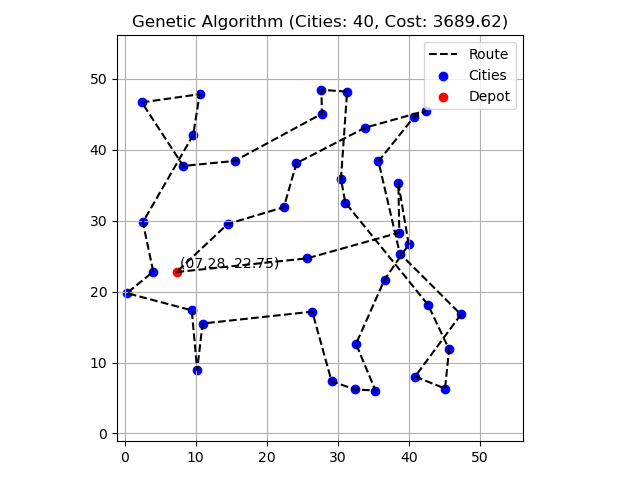
\includegraphics[width=\columnwidth,height=2.8cm]{images/img/separate/tsp/genetic_algorithm_040_3689_062.png}
		\captionof{figure}{Genetic Algorithm, mutation=None}
		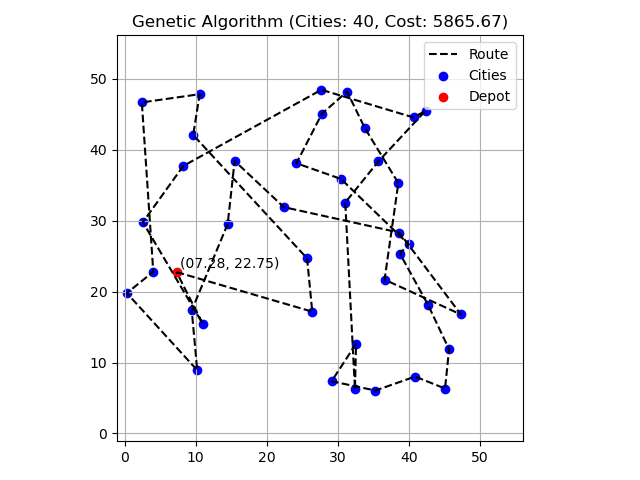
\includegraphics[width=\columnwidth,height=2.8cm]{images/img/tspgenetics/genetic-algorithm mutation=random-city-swap.png}
		\captionof{figure}{mutation=random-city-swap}
		\column{.4\textwidth}
		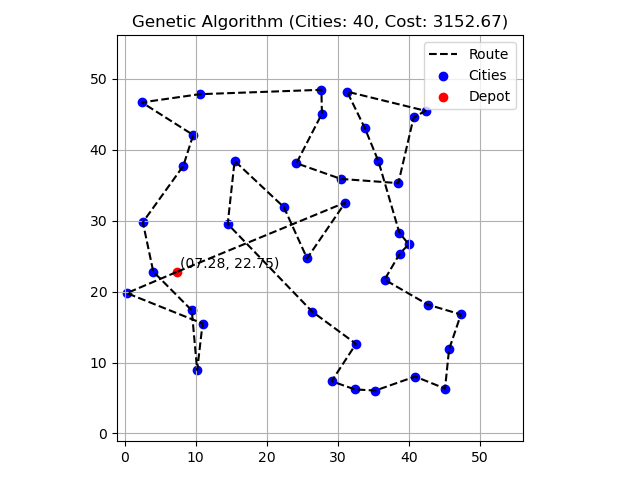
\includegraphics[width=\columnwidth,height=2.8cm]{images/img/tspgenetics/genetic-algorithm mutation=reverse-random-sublist.png}
		\captionof{figure}{mutation=reverse-random-sublist}
		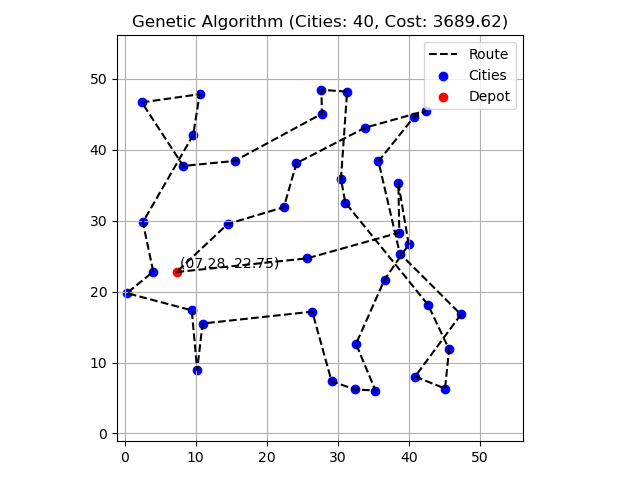
\includegraphics[width=\columnwidth,height=2.8cm]{images/img/tspgenetics/genetic-algorithm mutation=shift-1-move.png}
		\captionof{figure}{mutation=shift-1-move}
	\end{columns}
\end{frame}

\begin{frame}
	\frametitle{\el Υλοποίηση - \en TSP - chained}
	\begin{columns}[t]
		\column{.3\textwidth}
		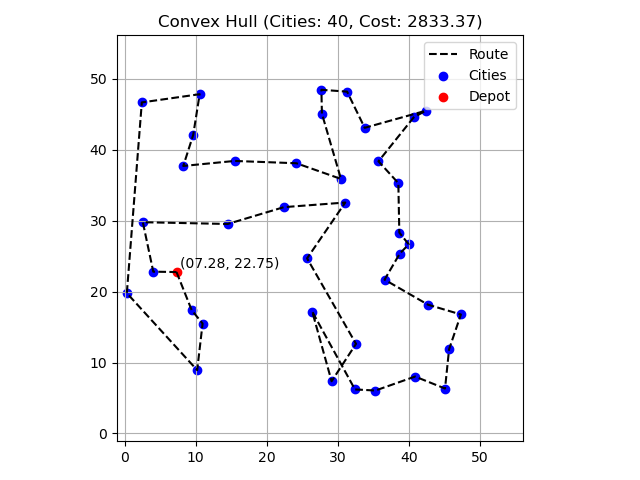
\includegraphics[width=\columnwidth,height=2.8cm]{images/img/chained/tsp/ac_sa_o2/convex_hull_040_2833_037.png}
		\captionof{figure}{Angle Comparison - Simulated Annealing - Opt-2 }
		\column{.3\textwidth}
		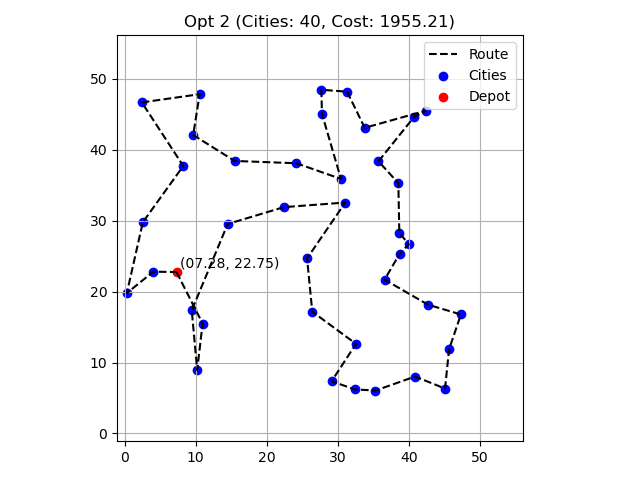
\includegraphics[width=\columnwidth,height=2.8cm]{images/img/chained/tsp/ac_sa_o2/opt_2_040_1955_020.png}
		\captionof{figure}{Angle Comparison - Simulated Annealing - Opt-2}
		\column{.3\textwidth}
		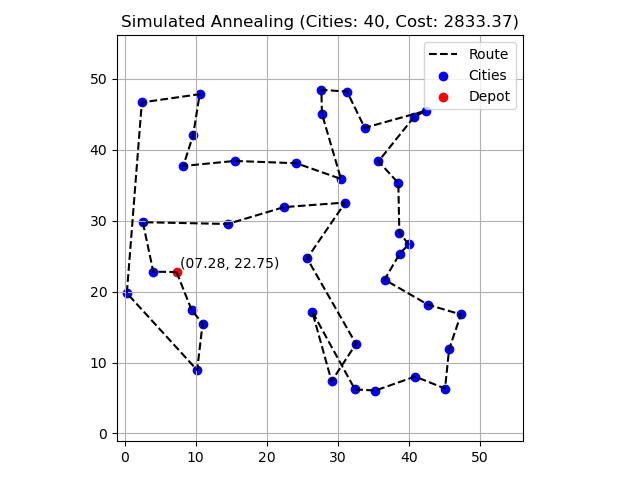
\includegraphics[width=\columnwidth,height=2.8cm]{images/img/chained/tsp/ac_sa_o2/simulated_annealing_040_2833_037.png}
		\captionof{figure}{Angle Comparison - Simulated Annealing - Opt-2}
	\end{columns}
\end{frame}

\begin{frame}
	\frametitle{\el Υλοποίηση - \en TSP - chained}
	\begin{columns}[t]
		\column{.3\textwidth}
		\includegraphics[width=\columnwidth,height=2.8cm]{images/img/chained/tsp/ec_sa_o2/convex_hull_040_1927_068.png}
		\captionof{figure}{Eccentricity Comparison - Simulated Annealing - Opt-2 }
		\column{.3\textwidth}
		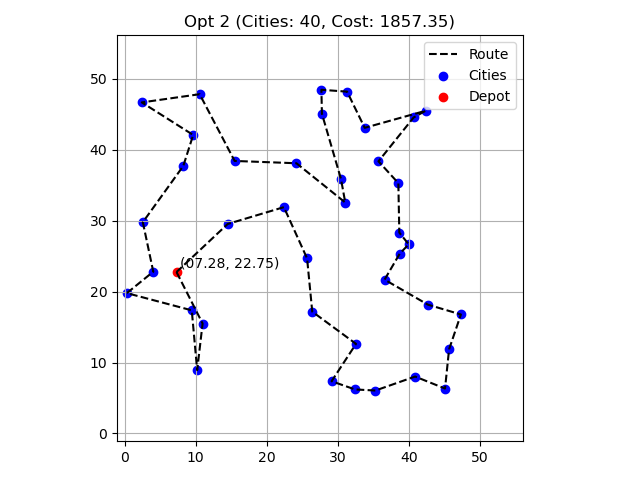
\includegraphics[width=\columnwidth,height=2.8cm]{images/img/chained/tsp/ec_sa_o2/opt_2_040_1857_035.png}
		\captionof{figure}{Eccentricity Comparison - Simulated Annealing - Opt-2}
		\column{.3\textwidth}
		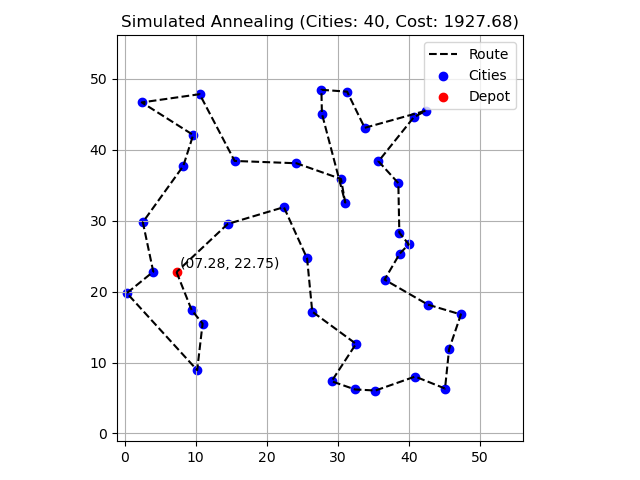
\includegraphics[width=\columnwidth,height=2.8cm]{images/img/chained/tsp/ec_sa_o2/simulated_annealing_040_1927_068.png}
		\captionof{figure}{Eccentricity Comparison - Simulated Annealing - Opt-2}
	\end{columns}
\end{frame}

\begin{frame}
	\frametitle{\el Υλοποίηση - \en TSP - chained}
	\begin{columns}[t]
		\column{.3\textwidth}
		\includegraphics[width=\columnwidth,height=2.8cm]{images/img/chained/tsp/nn_sa_o2/nearest_neighbor_040_4484_021.png}
		\captionof{figure}{Nearest Neighbor - Simulated Annealing - Opt-2 }
		\column{.3\textwidth}
		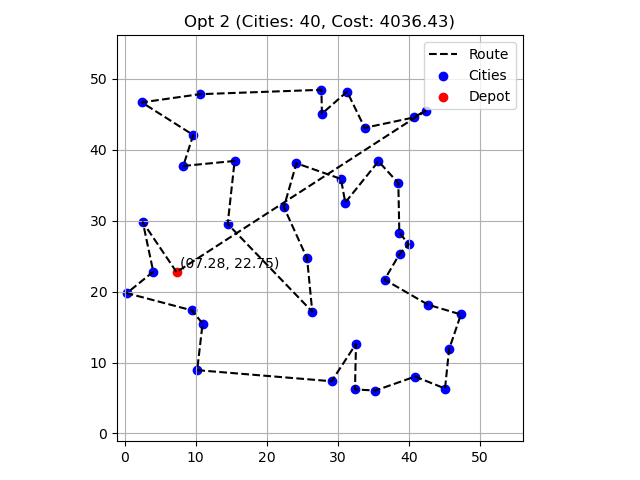
\includegraphics[width=\columnwidth,height=2.8cm]{images/img/chained/tsp/nn_sa_o2/opt_2_040_4036_043.png}
		\captionof{figure}{Nearest Neighbor - Simulated Annealing - Opt-2}
		\column{.3\textwidth}
		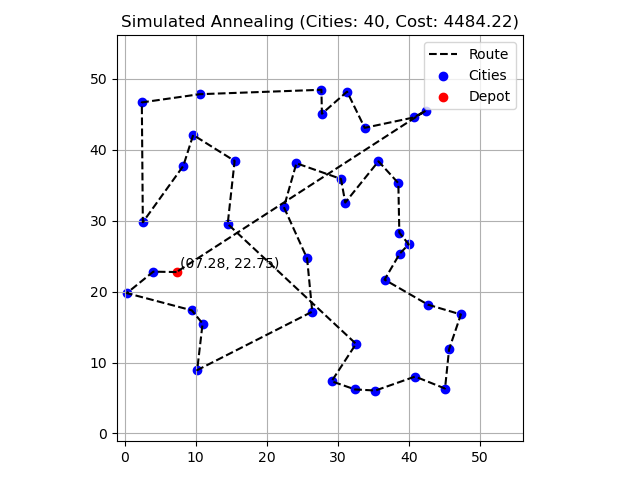
\includegraphics[width=\columnwidth,height=2.8cm]{images/img/chained/tsp/nn_sa_o2/simulated_annealing_040_4484_021.png}
		\captionof{figure}{Nearest Neighbor - Simulated Annealing - Opt-2}
	\end{columns}
\end{frame}

\begin{frame}
	\frametitle{\el Υλοποίηση - \en TWTSP}
	\begin{figure}
		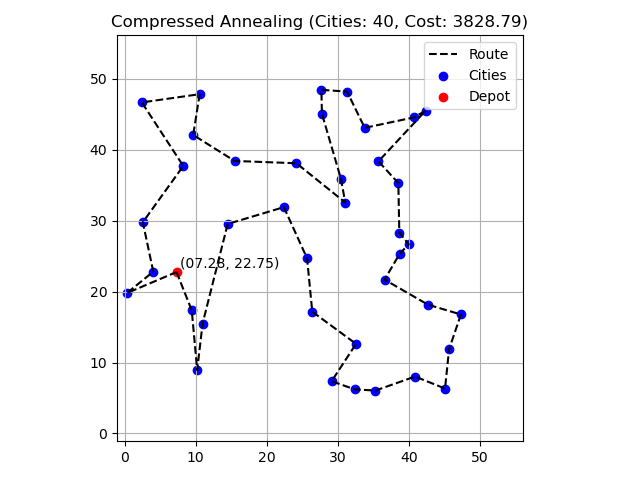
\includegraphics[scale=0.5]{images/img/separate/tsptw/compressed_annealing_040_3828_078.png}
		\captionof{figure}{Compressed Annealing}
	\end{figure}
\end{frame}

\begin{frame}
	\frametitle{\el Υλοποίηση - \en TWTSP}
	\begin{columns}[t]
		\column{.3\textwidth}
		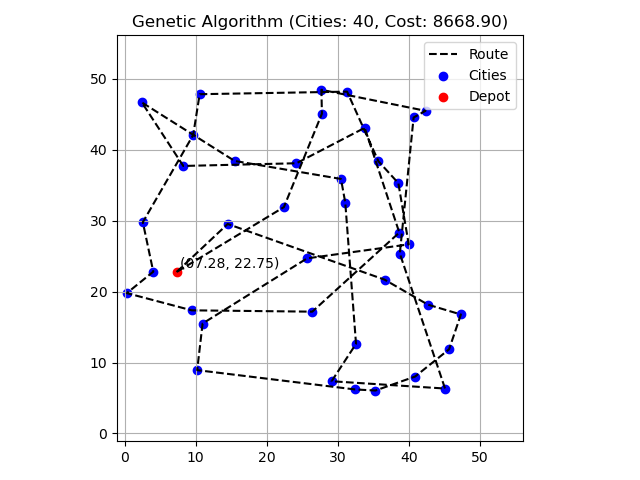
\includegraphics[width=\columnwidth,height=2.8cm]{images/img/tsptwgenetics/random-city-swap.png}
		\captionof{figure}{Genetic Algrithm - mutation=random-city-swap}
		\column{.3\textwidth}
		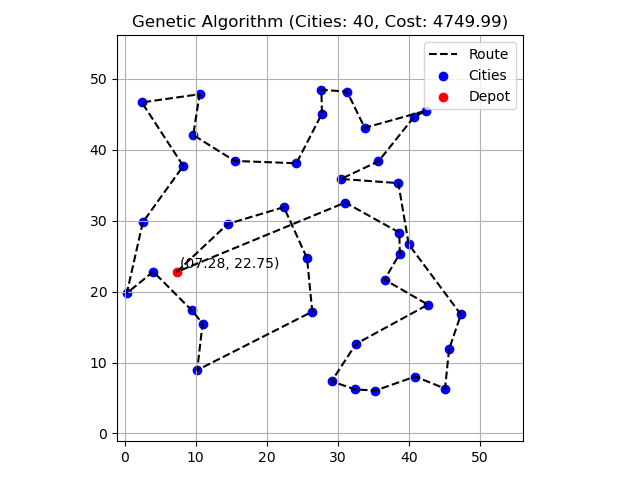
\includegraphics[width=\columnwidth,height=2.8cm]{images/img/tsptwgenetics/reverse-random-sublist.png}
		\captionof{figure}{Genetic Algrithm - mutation=reverse-random-sublist}
		\column{.3\textwidth}
		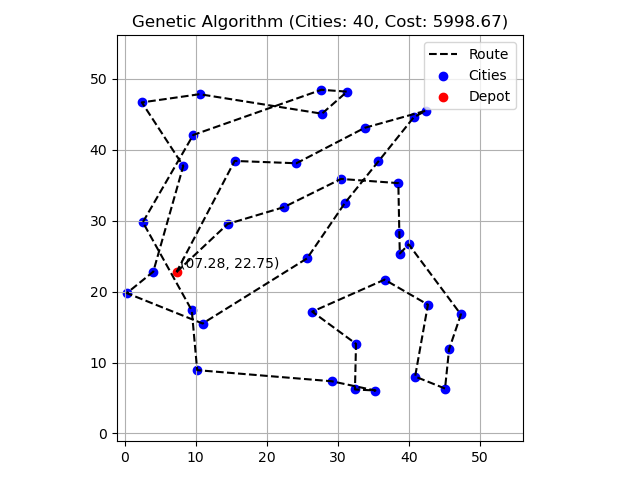
\includegraphics[width=\columnwidth,height=2.8cm]{images/img/tsptwgenetics/shift-1-move.png}
		\captionof{figure}{Genetic Algrithm - mutation=shift-1-move}
	\end{columns}
\end{frame}

\begin{frame}
	\frametitle{\el Υλοποίηση - \en TWTSP - chained}
	\begin{columns}[t]
		\column{.3\textwidth}
		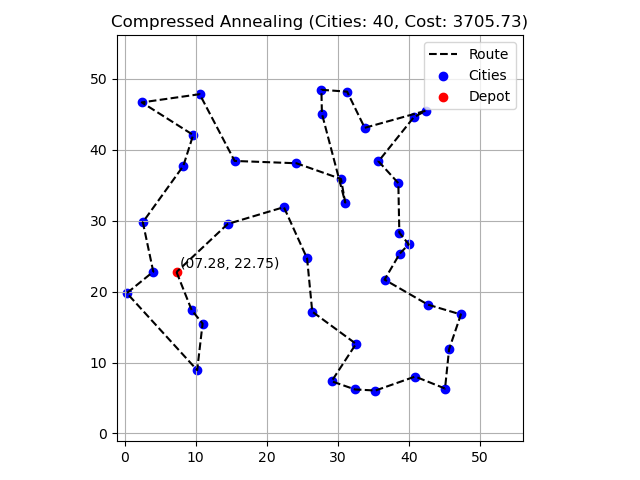
\includegraphics[width=\columnwidth,height=2.8cm]{images/img/chained/tsptw/ec_ca_opt2/compressed_annealing_040_3705_073.png}
		\captionof{figure}{Eccentricity Comparison - Compressed Annealing - Opt-2 }
		\column{.3\textwidth}
		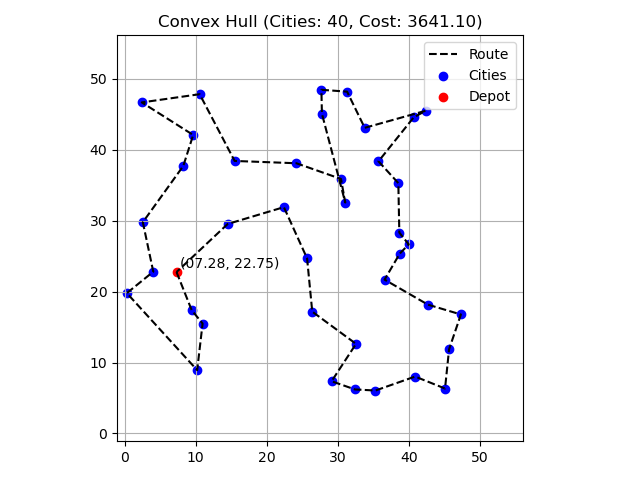
\includegraphics[width=\columnwidth,height=2.8cm]{images/img/chained/tsptw/ec_ca_opt2/convex_hull_040_3641_010.png}
		\captionof{figure}{Eccentricity Comparison - Compressed Annealing - Opt-2 }
		\column{.3\textwidth}
		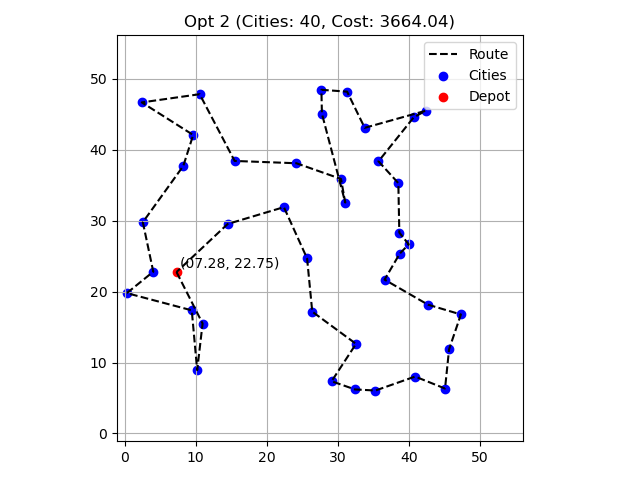
\includegraphics[width=\columnwidth,height=2.8cm]{images/img/chained/tsptw/ec_ca_opt2/opt_2_040_3664_003.png}
		\captionof{figure}{Eccentricity Comparison - Compressed Annealing - Opt-2 }
	\end{columns}
\end{frame}

\section{Discussion and Future work}
\begin{frame}
	\frametitle{\en Discussion and Future work}
	\footnotesize
	\tableofcontents[currentsubsection]
\end{frame}

\begin{frame}
	\frametitle{\en Discussion and Future work}
	\begin{itemize}
		\item \en Terrain Generation \el βασιζόμενο στο \en TSP \el με \en eccentricity comparison
		\item \el Εφαρμογή πραγματικού χρόνου για το \en Vehicle routing problem \en για σμήνος λεωφορείων. Σχετικό \en implementation μπορεί κανείς να αναζητήσει στο \en GitHub Repository: \url{https://github.com/billsioros/MMGP}
		\item \el Μελέτη των δυνατοτήτων του \en TSP \el για \en racing games \el όπως το \en Βurnout paradise
	\end{itemize}
	\begin{figure}
		
\includegraphics[scale=0.2]{images/Burnout_Paradise.jpg}
		\caption{Burnout Paradise\\ πηγή: \url{https://en.wikipedia.org/wiki/Burnout_Paradise}}
	\end{figure}
\end{frame}

\section{Βιβλιογραφία}
\begin{frame}
	\frametitle{Βιβλιογραφία}
	\footnotesize
	\begin{thebibliography}{depth}
		\setbeamertemplate{bibliography item}[text]
		\bibitem[1]{1}
		Exact and Approximation Algorithms for Time-Window TSP, 
		Jie Gao, Su Jia, Joseph S. B. Mitchell,
		CG:YRF, Boston, MA, USA, June 14-18, 2016
		
		\bibitem[2]{2}
		A Compressed-Annealing Heuristic for the Traveling Salesman Problem with Time Windows, 
		Jeffrey W. Ohlmann, Barrett W. Thomas,
		INFORMS Journal on Computing,
		Vol. 19, No. 1, Winter 2007, pp. 80–90
		
		\bibitem[3]{3}
		An Effective Heuristic Algorithm for the Traveling-Salesman Problem,
		S. Lin, B. W. Kernighan,
		October 1971
		
		\bibitem[4]{4}
		Εισαγωγή στους αλγορίθμους, Δεύτερη έκδοση, 
		Thomas H. Cormen, Charles E. Leiserson, Ronald L. Rivest, Clifford Stein,
		Πανεπιστημιακές εκδόσεις Κρήτης, 2011,
		ISBN: 978-960-524-473-6
		
		\bibitem[5]{5}
		Τεχνητή Νοημοσύνη, Μία σύγχρονη προσέγγιση, Δεύτερη Αμερικανική έκδοση, 
		Stuart Russel, Peter Norvig,
		σελ.: 101,
		Κλειδάριθμος 2005,
		ISBN: 960-209-873-2
		
		\bibitem[6]{6}
		Στοιχεία διακριτών μαθηματικών, 
		C. L. Liu,
		σελ.: 171-172, 178-179, 190-201,
		Πανεπιστημιακές εκδόσεις Κρήτης 2014, 
		ISBN: 978-960-524-072-1	
	\end{thebibliography}
\end{frame}

\begin{frame}
	\frametitle{Βιβλιογραφία}
	\footnotesize
	\begin{thebibliography}{depth}
		\setbeamertemplate{bibliography item}[text]
		
		\bibitem[7]{7}
		Discrete and Computational Geometry, 
		Satyan L. Devadoss, Joseph O'Rourke,
		σελ.: 81-86,
		Princeton University Press, 2011, 
		ISBN: 978-0-691-14553-2
		
		\bibitem[8]{8}
		Computational Geometry,	Algorithms and Applications, Third Edition, 
		Mark de Berg, Otfried Cheong, Marc van Kreveld, Mark Overmars,
		σελ.: 193-204,
		Springer, 2008, 
		ISBN: 978-3-540-77973-5
		
		\bibitem[9]{9}
		Υπολογιστική Γεωμετρία: Μια σύγχρονη αλγοριθμική προσέγγιση, 
		Γιάννης Ζ. Εμίρης,
		σελ.: 95-100, 103-107, 199-208,
		Κλειδάριθμος, 2008, 
		ISBN: 978-960-461-141-6 
		
		\bibitem[10]{10}
		An O ( n log n ) Heuristic for the Euclidean Traveling Salesman Problem, 
		Evgeny Yanenko, Eckart
		Schuhmacher, Ulrich Spörlein, Kurt Tutschku,
		April 25, 2005
		
		\bibitem[11]{11}
		Applications of the TSP,
		http://www.math.uwaterloo.ca/tsp/apps/index.html
		
		\bibitem[12]{12}
		Approximation Algorithms for Time-Window
		TSP and Prize Collecting TSP Problems,
		Jie Gao, Su Jia, Joseph S. B. Mitchell, Lu Zhao,
		Stony Brook University, Stony Brook, NY 11794, USA
	\end{thebibliography}
\end{frame}

\begin{frame}
	\frametitle{Βιβλιογραφία}
	\footnotesize
	\begin{thebibliography}{depth}
		\setbeamertemplate{bibliography item}[text]
		
		\bibitem[13]{13}
		Good triangulations yield good tours,
		Adam N. Letchford, Nicholas A. Pearson,
		Department of Management Science, Lancaster University, Lancaster LA1 4YW, UK, 
		4 May 2006
		
		\bibitem[14]{14}
		Σχεδίαση και Ανάλυση Αλγορίθμων,
		Κωνσταντίνος Τσίχλας, Ιωάννης Μανωλόπουλος, Αναστάσιος Γούναρης,
		σελ.: 317-320,
		http://repfiles.kallipos.gr/html\_books/4410/contents.html ,2015
		ISBN: 978-960-603-465-7
		
		\bibitem[15]{15}
		Μαθηματικά Πληροφορικής,
		Ηλίας Κουτσουπιάς,
		σελ.: 112,
		Πανεπιστήμιο Αθηνών, Αθήνα, Οκτώβριος 2009
		
		\bibitem[16]{16}
		Geometric Approaches to solving the traveling salesman problem,
		John P. Norback, Robert F. Love,
		Managment Science, Vol. 23, No. 11,σελ.: 1208-1223,
		Ιούλιος 1977
		
		\bibitem[17]{17}
		The Convex-Hull-and-Line
		Traveling Salesman Problem: A Solvable Case,
		Vladimir G. Deineko, Rene van Dal, Gunter Rote,
		Information Processing Letters 51 (1994), σελ.: 141-148,
		Σεπτέμβριος 1992
		
		\bibitem[18]{18}
		Traveling Salesman Cycles are not always subgraphs of Delaunay triangulations or of Minimum weight triangulations,	Michael B. DILLENCOURT,
		Computer Technology Associates, Inc.
	\end{thebibliography}
\end{frame}

\end{document}